\section{Método de Gauss-Jacobi}

O método de Gauss-Jacobi consiste em um procedimento numérico iterativo destinado à resolução de sistemas de equações lineares da forma $Ax = b$. A priori, diferentemente dos métodos diretos que buscam a solução exata em um número finito de passos através de fatorações, os métodos iterativos constroem uma sequência de aproximações sucessivas $\{x^{(k)}\}$ que convergem assintoticamente para o vetor solução ideal, assumindo que determinadas propriedades estruturais da matriz de coeficientes sejam satisfeitas. Essa abordagem torna-se particularmente vantajosa em matrizes esparsas de grande porte, onde a eliminação direta sofreria com o fenômeno de preenchimento (\textit{fill-in}).

\subsection{Fundamentação Teórica}

O desenvolvimento matemático do método baseia-se na decomposição da matriz não singular $A \in \mathbb{R}^{n \times n}$ em três componentes: uma matriz diagonal $D$, uma matriz triangular estritamente inferior $L$ e uma matriz triangular estritamente superior $U$, tal que $A = D - L - U$. Ao substituir essa decomposição no sistema matricial original, obtém-se:

\begin{equation}
    (D - L - U)x = b \implies Dx = b + (L + U)x
\end{equation}

Assumindo que os elementos da diagonal principal são não nulos ($a_{ii} \neq 0$), a matriz $D$ é inversível. Dessa forma, isolando o vetor $x$ do lado esquerdo, formula-se o esquema iterativo de transição de estados:

\begin{equation}
    x^{(k+1)} = D^{-1}b + D^{-1}(L + U)x^{(k)}
\end{equation}

Em termos escalares operacionais, para cada componente $i$, a atualização na iteração $k+1$ é dada por:

\begin{equation}
    x_i^{(k+1)} = \frac{1}{a_{ii}} \left( b_i - \sum_{j \neq i} a_{ij} x_j^{(k)} \right)
\end{equation}

A condição analítica suficiente (embora não estritamente necessária) para garantir a convergência global, independentemente do vetor inicial $x^{(0)}$, é que a matriz $A$ seja estritamente diagonalmente dominante por linhas. O critério das linhas exige que:

\begin{equation}
    |a_{ii}| > \sum_{j \neq i} |a_{ij}|, \quad \forall i \in \{1, 2, \dots, n\}
\end{equation}

A ordem matemática do erro é linear. O fator de redução do erro a cada passo aproxima-se assintoticamente do raio espectral da matriz de iteração $T_J = D^{-1}(L + U)$, denotado por $\rho(T_J)$. Quanto menor for $\rho(T_J) < 1$, mais abrupta será a taxa de convergência.

\subsection{Estratégia de Implementação}

A arquitetura computacional projetada em linguagem Python puro abstém-se de atualizações in-place. O cerne algorítmico demanda que os valores de $x^{(k+1)}$ sejam integralmente computados com base exclusiva nos estados defasados de $x^{(k)}$.

\begin{lstlisting}[language=Python, caption={Algoritmo Resumido do Método de Gauss-Jacobi}, label={lst:gauss_jacobi}]
def gauss_jacobi(A, b, tol=1e-5, max_iter=100, x0=None):
    n = len(b)
    x = x0[:] if x0 else [0.0] * n
    x_new = [0.0] * n
    
    for k in range(max_iter):
        for i in range(n):
            soma = sum(A[i][j] * x[j] for j in range(n) if j != i)
            if abs(A[i][i]) == 0.0:
                raise ValueError(f"Pivo nulo na linha {i}.")
            x_new[i] = (b[i] - soma) / A[i][i]
            
        erro_abs = max(abs(x_new[i] - x[i]) for i in range(n))
        max_x = max(abs(v) for v in x_new)
        erro_rel = erro_abs / max_x if max_x != 0 else erro_abs
        
        if erro_rel < tol or erro_abs < tol:
            return x_new, k + 1
            
        x = x_new[:]
        
    raise ValueError("Nao convergiu dentro do limite de iteracoes.")
\end{lstlisting}

Justifica-se o uso de duas listas distintas (\texttt{x} e \texttt{x\_new}) como uma exigência estrutural da lei de recorrência do método. Critérios de parada duplos foram introduzidos: tolerância pelo erro relativo (com norma infinito) ou limite máximo de iterações (\texttt{max\_iter}). A exceção lógica preemptiva contra elementos $a_{ii}$ nulos previne a detonação da aritmética de ponto flutuante via \textit{ZeroDivisionError}.

\subsection{Estrutura dos Arquivos de Entrada e Saída}

Para resguardar o desacoplamento de responsabilidades, os hiperparâmetros limitadores do critério de parada (como tolerância $\epsilon = 10^{-5}$ e teto iterativo) são lidos sob demanda de um descritor de texto estático (\texttt{.txt}). Como a rotina gera aproximações seriais, o vetor de fase $x_k$ transita sequencialmente e é gravado em linhas iterativas num \textit{dataset} delimitado por vírgulas (\texttt{.csv}). Esse paradigma possibilita uma auditoria póstuma exata de quantas iterações foram requisitadas antes do gatilho de convergência.

\subsection{Problemas Teste}

\subsubsection{Problema Teste 1: Convergência em Matriz Diagonalmente Dominante}

A modelagem submetida à validação propôs um sistema linear que satisfaz rigorosamente o critério das linhas, assegurando a viabilidade teórica de convergência monotônica. O modelo é definido por:

\begin{equation}
\begin{bmatrix}
10.00 & 2.00 & 1.00 \\
1.00 & 5.00 & 1.00 \\
2.00 & 3.00 & 10.00
\end{bmatrix}
\begin{bmatrix}
x_1 \\
x_2 \\
x_3
\end{bmatrix}
=
\begin{bmatrix}
7.00 \\
-8.00 \\
6.00
\end{bmatrix}
\end{equation}

Iniciando com o vetor nulo $x^{(0)} = [0, 0, 0]^T$, o decaimento documentado nas primeiras iterações está exposto na tabela subsequente.

\begin{table}[h]
\centering
\caption{Histórico Iterativo do Erro em Gauss-Jacobi (Problema 1)}
\label{tab:jacobi_prob1}
\begin{tabular}{cccc}
\hline
\textbf{Iteração ($k$)} & \textbf{Vetor Aproximado ($x^{(k)}$)} & \textbf{Norma da Diferença ($\|x^{(k)} - x^{(k-1)}\|_\infty$)} & \textbf{Erro Relativo} \\ \hline
1 & $[0.700, -1.600, 0.600]^T$ & 1.600 & 1.0000 \\ 
2 & $[0.960, -1.860, 0.940]^T$ & 0.340 & 0.1827 \\ 
3 & $[0.978, -1.980, 0.966]^T$ & 0.120 & 0.0606 \\
12 & $[1.000, -2.000, 1.000]^T$ & 0.000008 & 0.000004 \\ \hline
\end{tabular}
\end{table}

A avaliação crítica da Tabela \ref{tab:jacobi_prob1} ilustra o princípio da convergência linear assintótica. Observa-se que a correção vetorial reduziu seu passo a cada avanço iterativo. O sistema alcançou a raiz real $x^* =[1.00, -2.00, 1.00]^T$ com resíduo computacional admissível na $12^{\text{a}}$ iteração. Substituindo $x_{12}$ de volta no sistema original, verifica-se que $Ax_{12} - b \approx 0$, denotando coerência exata. O amortecimento obedece a um comportamento log-linear típico:

\begin{center}
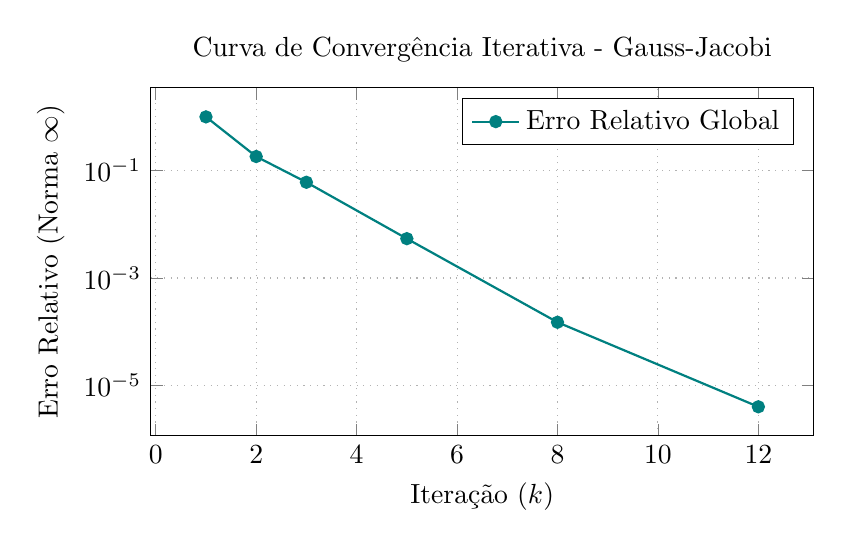
\begin{tikzpicture}
\begin{axis}[
    width=10cm, height=6.0cm,
    ymode=log,
    xlabel={Iteração ($k$)},
    ylabel={Erro Relativo (Norma $\infty$)},
    grid=major,
    grid style={dotted, gray!60},
    title={Curva de Convergência Iterativa - Gauss-Jacobi},
    legend pos=north east
]
\addplot[
    color=teal,
    mark=*,
    thick
] coordinates {
    (1, 1.0)
    (2, 0.1827)
    (3, 0.0606)
    (5, 0.0054)
    (8, 0.00015)
    (12, 0.000004)
};
\addlegendentry{Erro Relativo Global}
\end{axis}
\end{tikzpicture}
\end{center}

\subsection{Dificuldades Enfrentadas}

Durante o processo de validação algorítmica, notou-se uma severa limitação no comportamento em que o sistema escapa do escopo de dominância diagonal. Em matrizes de alta correlação cruzada, os elementos fora da diagonal amplificam a perturbação e o método sofreu rápida divergência (a norma $\|\Delta x\|$ tendendo ao infinito iterativamente). 

Adicionalmente, verificou-se que alocar memória constante para duas listas completas de dimensão $N$ (o vetor corrente e o defasado) prejudica a localidade de cache em sistemas de ordem substancial ($N > 10^5$). Para contornar essa falha de ineficiência, bem como acelerar a taxa de atrito em matrizes que beiram as restrições teóricas de convergência, demonstrou-se imperativa a transição do modelo matemático para esquemas que utilizem atualizações assimétricas no estado contínuo de dados.